% !TeX root = ../main.tex

% Edit this title for each week's entry.
\section{Week 6 - Comparison Methods (Part 2)}

\topic{Internal Rate of Return}

\heading{Rate of Return Analysis}
Cash-flow equivalence methods (PW, AW) require us to know the discount rate
\dbb{before} we start. \rb{Rate of return analysis} instead \emph{starts}
by asking what \emph{is} the rate of return on an investment. Compare:
\begin{itemize}
    \item ``The present worth of this project is \$32,000''
    \item ``The annual worth of this project is \$2,800''
    \item ``The project will produce a 23\% rate of return''
\end{itemize}

\begin{example}[Rate of Return]
    If \$100 is invested today in a project that returns \$110 next year,
    what is the rate of return?
    \begin{center}
        \begin{tikzpicture}[scale=0.8]
            \draw[->] (0,0) -- (3,0) node[right] {\scriptsize Year};
            \node[below left] at (0,0) {\scriptsize 0};
            \node[below] at (2,-0.05) {\scriptsize 1};
            \draw[->,thick,red!70!black] (0,0) -- (0,-1) node[below] {\scriptsize \$100};
            \draw[->,thick,blue!70!black] (2,0) -- (2,1.1) node[above] {\scriptsize \$110};
        \end{tikzpicture}
    \end{center}
    \[P = F(P/F,i^*,1) \;\Rightarrow\; 100 = \frac{110}{1+i^*} \;\Rightarrow\; i^* = \db{10\%}\]
    \db{A 10\% rate makes the PW of benefits equal to the PW of costs/investments.}
\end{example}

\begin{definition}[Internal Rate of Return (IRR)]
    The discount rate at which the \dbb{present worth of a project is equal
    to 0}:
    \[\boxed{\begin{gathered}
        \text{PW}(i^*) = \sum_{t=0}^{N} \frac{F_t}{(1+i^*)^t} = 0\\[4pt]
        \begin{array}{@{}l@{}}
            i^*: \text{internal rate of return}\\
            F_t: \text{net cash-flow at time } t\\
            N: \text{project life (periods)}
        \end{array}
    \end{gathered}}\]
    Equivalently, the discount rate that makes
    \[\text{PW(benefits)} = \text{PW(costs)} \quad\text{or}\quad \text{AW(benefits)} = \text{AW(costs)}\]
    More profitable projects $\to$ \dbb{higher IRR}.
\end{definition}

\begin{example}[IRR of an Investment Project]
    Find the IRR of the following project (cash-flows in \$K).
    \begin{center}
        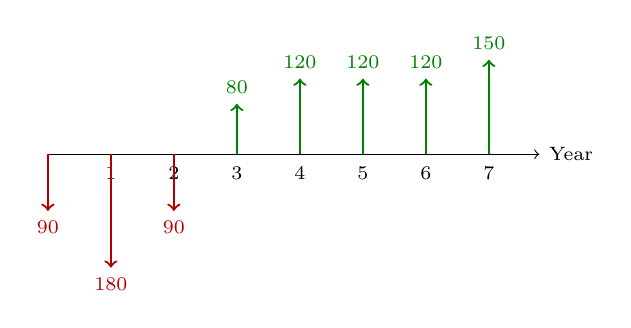
\begin{tikzpicture}[scale=0.8]
            \draw[->] (0,0) -- (7.8,0) node[right] {\scriptsize Year};
            \foreach \x in {1,...,7}{\node[below] at (\x,-0.05) {\scriptsize \x};}
            \draw[->,thick,red!70!black] (0,0) -- (0,-0.9) node[below] {\scriptsize 90};
            \draw[->,thick,red!70!black] (1,0) -- (1,-1.8) node[below] {\scriptsize 180};
            \draw[->,thick,red!70!black] (2,0) -- (2,-0.9) node[below] {\scriptsize 90};
            \draw[->,thick,green!50!black] (3,0) -- (3,0.8) node[above] {\scriptsize 80};
            \foreach \x in {4,5,6}{\draw[->,thick,green!50!black] (\x,0) -- (\x,1.2) node[above] {\scriptsize 120};}
            \draw[->,thick,green!50!black] (7,0) -- (7,1.5) node[above] {\scriptsize 150};
        \end{tikzpicture}
    \end{center}
    \begin{align*}
        \text{PW}(i) = -90 &- \frac{180}{1+i} - \frac{90}{(1+i)^2} + \frac{80}{(1+i)^3}\\
        &+ \frac{120}{(1+i)^4} + \frac{120}{(1+i)^5} + \frac{120}{(1+i)^6} + \frac{150}{(1+i)^7}
    \end{align*}
    \db{There is no closed form, so estimate. Evaluate PW at a few rates (with $(P/F,i,N)$ factors):}
    \begin{center}
    \begin{tabular}{cccccc}
        \toprule
        $i$ & 0\% & 5\% & 10\% & 15\% & 20\% \\
        \midrule
        PW (\$K) & 230.0 & 114.9 & 33.3 & $-25.4$ & $-68.1$ \\
        \bottomrule
    \end{tabular}
    \end{center}
    \db{PW changes sign between 10\% and 15\%. Linear interpolation:}
    \[i^* \approx 10\% + 5\% \cdot \frac{33.3}{33.3 - (-25.4)} = 12.8\%\]
    \db{The exact value (Excel) is $i^* = \dbb{12.63\%}$. Interpolation slightly overestimates because the curve is convex.}
\end{example}

\begin{center}
    \begin{tikzpicture}
        \draw[->] (0,0) -- (10.8,0) node[right] {\scriptsize $i$};
        \draw[->] (0,-1) -- (0,3.2) node[above] {\scriptsize PW (\$K)};
        \foreach \p in {5,10,15,20}{\draw ({\p*0.4},0.06) -- ({\p*0.4},-0.06) node[below] {\scriptsize \p\%};}
        \foreach \v in {-50,50,100,150,200}{\draw (0.06,{\v*0.012}) -- (-0.06,{\v*0.012}) node[left] {\scriptsize \v};}
        \draw[thick,red,domain=0:0.25,samples=60] plot ({\x*40},{0.012*(-90-180/(1+\x)-90/(1+\x)^2+80/(1+\x)^3+120/(1+\x)^4+120/(1+\x)^5+120/(1+\x)^6+150/(1+\x)^7)});
        \fill (5.05,0) circle (1.5pt) node[above right] {\scriptsize IRR $= 12.63\%$};
    \end{tikzpicture}
    \\[2pt] \textit{\small For simple investments (costs earlier than benefits), higher $i$ gives lower PW}
\end{center}

\heading{Using MS Excel to Find IRR}
\begin{itemize}
    \item \rb{NPV}: finds the present worth, \texttt{=NPV(i, cash flows)}. NB: it \dbb{starts with year 1}! Add the year-0 cash-flow separately
    \item \rb{IRR}: finds the IRR, \texttt{=IRR(cash flows, guess)}. Include the year-0 cash-flow
\end{itemize}
\begin{center}
\begin{tabular}{clll}
    \toprule
    & A & B & C \\
    \midrule
    1 & Year & Cash flow & \\
    2--9 & 0, 1, \dots, 7 & $-90$, $-180$, \dots, 150 & \\
    11 & IRR & 12.63\% & \texttt{=IRR(B2:B9,12\%)} \\
    13 & PW & \$0.0 & \texttt{=B2+NPV(12.63\%,B3:B9)} \\
    14 & PW & \$114.94 & \texttt{=B2+NPV(5\%,B3:B9)} \\
    \bottomrule
\end{tabular}
\end{center}

\begin{example}[IRR: Analytical Solution]
    \$5,000 is invested today in a project that returns \$5,500 in 2 years.
    What is the IRR?
    \\\db{Only two cash-flows, so solve directly:}
    \[5000 = 5500(P/F,i^*,2) = \frac{5500}{(1+i^*)^2} \;\Rightarrow\; i^* = \sqrt{1.1} - 1 = \db{4.88\%}\]
\end{example}

\begin{definition}[Simple Investment]
    A project where \dbb{all negative cash-flows occur before all positive
    cash-flows}. For simple investments, evaluating an \b{independent}
    project with IRR:
    \begin{itemize}
        \item $\text{IRR} > \text{MARR} \to$ worthwhile ($\text{PW} > 0$)
        \item $\text{IRR} < \text{MARR} \to$ not worthwhile ($\text{PW} < 0$)
    \end{itemize}
\end{definition}
\db{In the investment project above: at MARR $= 5\% < 12.63\%$, $\text{PW} = \$114.94\text{K} > 0$. The PW curve is decreasing, so $\text{IRR} > \text{MARR} \iff \text{PW(MARR)} > 0$.}

\heading{Limitation of IRR: Not a Simple Investment}
\begin{itemize}
    \item When cash-flows change sign ($+ \to -$ or $- \to +$) \dbb{more than once}, calculating IRR becomes complicated
    \item There can be \dbb{multiple} discount rates that make $\text{PW} = 0$
\end{itemize}

\begin{example}[Not a Simple Investment]
    Year 0: $+1000$; Year 1: $-2500$; Year 2: $-2500$; Year 3: $+6000$.
    \\\db{The signs go $+ \to - \to +$ (two changes). Set $x = 1 + i$:}
    \[1000x^3 - 2500x^2 - 2500x + 6000 = 0 \;\Rightarrow\; (x - 1.5)(x^2 - x - 4) = 0\]
    \[x = 1.5 \text{ or } x = \tfrac{1 + \sqrt{17}}{2} = 2.562 \;\Rightarrow\; i^* = \db{50\%} \text{ and } i^* = \db{156\%}\]
    \db{(The third root $x < 0$ is not a meaningful rate.) Which one is ``the'' IRR? Neither is a useful measure of profitability.}
    \begin{center}
        \begin{tikzpicture}
            \draw[->] (0,0) -- (8.8,0) node[right] {\scriptsize $i$};
            \draw[->] (0,-0.6) -- (0,3.3) node[above] {\scriptsize PW};
            \foreach \p in {50,100,150,200}{\draw ({\p*0.04},0.06) -- ({\p*0.04},-0.06) node[below] {\scriptsize \p\%};}
            \foreach \v in {500,1000}{\draw (0.06,{\v*0.0025}) -- (-0.06,{\v*0.0025}) node[left] {\scriptsize \v};}
            \draw[thick,blue!70!black,domain=0.1:2,samples=80] plot ({\x*4},{0.0025*(1000-2500/(1+\x)-2500/(1+\x)^2+6000/(1+\x)^3)});
            \fill (2,0) circle (1.5pt) node[above right] {\scriptsize 50\%};
            \fill (6.246,0) circle (1.5pt) node[above left] {\scriptsize 156\%};
        \end{tikzpicture}
    \end{center}
\end{example}

\heading{Summary}
\begin{enumerate}
    \item \b{IRR}: the discount rate that makes $\text{PW} = 0$
    \item For simple investments, IRR is a useful measure of profitability. For independent projects, compare IRR to MARR
    \item IRR is useful for \b{simple investments only}: if cash-flows change sign more than once, there can be multiple IRRs
\end{enumerate}

\topic{Comparing Mutually Exclusive Projects Using IRR}

\heading{Comparing Mutually Exclusive Options}
IRR is an \dbb{efficiency} (rate) of earning money, but it can be
misleading when comparing mutually exclusive options.

\begin{example}[Reflection: Higher IRR?]
    Project A has an IRR of 50\%; project B has an IRR of 40\%. The two
    projects are mutually exclusive. Which option is better?
    \\\db{We can't tell from IRR alone: it says nothing about how much money is invested.}
\end{example}

\begin{example}[Reflection: Lending to George]
    You have \$20 and your friend George wants to borrow some money. You
    can either:
    \begin{enumerate}[label = \Alph*.]
        \item Lend him \$10 and receive \$15 in return (1 year); or
        \item Lend him \$20 and receive \$28 in return (1 year)
    \end{enumerate}
    MARR is 10\%. Which option should you choose?
    \begin{align*}
        \text{A: } & \text{IRR} = 15/10 - 1 = 50\%, & \text{PW} &= -10 + 15/1.1 = \$3.64\\
        \text{B: } & \text{IRR} = 28/20 - 1 = 40\%, & \text{PW} &= -20 + 28/1.1 = \$5.45
    \end{align*}
    \db{A has the higher IRR, but B leaves you better off. With A, the other \$10 only earns MARR. Look at the \dbb{increment} B $-$ A: lend an extra \$10 now, get an extra \$13 back:}
    \[\text{IRR}_{B-A} = 13/10 - 1 = 30\% > 10\% \;\Rightarrow\; \dbb{choose B}\]
\end{example}

\begin{remark}
    A higher IRR does not mean a better project: IRR is a rate of earning
    money, and just looking at it \textbf{ignores the size of the initial
    investment}.
\end{remark}

\begin{definition}[Incremental IRR]
    The IRR of the \dbb{difference} (the ``increment'') between two mutually
    exclusive alternatives. Steps in incremental analysis:
    \begin{enumerate}
        \item Order alternatives in \b{increasing order of first cost}
        \item Start with the ``do nothing'' alternative as the current best
        \item One by one, evaluate each alternative against the \b{best alternative found so far}: compute the IRR of (challenger $-$ current best)
        \begin{itemize}
            \item $\text{IRR}_\Delta > \text{MARR} \to$ the extra investment is worthwhile; the challenger becomes the current best
            \item $\text{IRR}_\Delta < \text{MARR} \to$ keep the current best
        \end{itemize}
        \item Repeat step 3 until all alternatives are evaluated
    \end{enumerate}
\end{definition}

\begin{example}[IRR of Mutually Exclusive Projects]
    ABC company must purchase a new lathe. It is considering 4 lathes with
    a 10-year lifetime and no salvage value. Which should be taken with a
    MARR of 15\%?
    \\\db{Order by increasing first cost:}
    \begin{center}
    \begin{tabular}{cccc}
        \toprule
        Lathe & First cost & Annual savings & IRR (alone) \\
        \midrule
        1 & 100,000 & 25,000 & 21.4\% \\
        2 & 150,000 & 34,000 & 18.5\% \\
        3 & 200,000 & 46,000 & 18.9\% \\
        4 & 255,000 & 55,000 & 17.1\% \\
        \bottomrule
    \end{tabular}
    \end{center}
    \db{Each increment is a first cost $\Delta P$ followed by 10 annual savings $\Delta A$, so solve $(P/A,i^*,10) = \Delta P/\Delta A$:}
    \begin{center}
    \begin{tabular}{lcccc}
        \toprule
        Comparison & $\Delta P$ & $\Delta A$ & $\text{IRR}_\Delta$ & Decision \\
        \midrule
        1 vs.\ do nothing & 100,000 & 25,000 & 21.4\% $>$ 15\% & take 1 \\
        2 vs.\ 1 & 50,000 & 9,000 & 12.4\% $<$ 15\% & keep 1 \\
        3 vs.\ 1 & 100,000 & 21,000 & 16.4\% $>$ 15\% & take 3 \\
        4 vs.\ 3 & 55,000 & 9,000 & 10.1\% $<$ 15\% & keep 3 \\
        \bottomrule
    \end{tabular}
    \end{center}
    \db{\dbb{Choose lathe 3}, even though lathe 1 has the highest IRR. Check with PW at 15\%, using $(P/A,15\%,10) = 5.0188$:}
    \[\text{PW}_1 = \$25{,}469, \quad \text{PW}_2 = \$20{,}638, \quad \text{PW}_3 = \db{\$30{,}863}, \quad \text{PW}_4 = \$21{,}032\]
    \db{Lathe 3 has the highest PW, so the two methods agree.}
\end{example}

\heading{Summary}
\begin{enumerate}
    \item When comparing \b{mutually exclusive} options, simply comparing IRRs ignores the size of the initial investment and may lead to the \b{wrong conclusion}
    \item Use \b{incremental IRR} instead: it gives the same choice as PW
\end{enumerate}

\topic{Payback Period}

\begin{definition}[Payback Period]
    The time it takes for an investment to be \dbb{recouped}: sum the
    revenues/savings until they equal the initial investment.
\end{definition}

\begin{definition}[Discounted Payback Period]
    Sum the \dbb{PW} of the revenues/savings (discounted at MARR) until they
    equal the initial investment.
\end{definition}

\begin{example}[Payback Period]
    Find the payback period for the following cash-flows. First cost
    $= \$100{,}000$.
    \begin{center}
    \begin{tabular}{ccc}
        \toprule
        $N$ & Cash-flow & \db{Cumulative} \\
        \midrule
        1 & \$10,000 & \db{\$10,000} \\
        2 & \$20,000 & \db{\$30,000} \\
        3 & \$25,000 & \db{\$55,000} \\
        4 & \$30,000 & \db{\$85,000} \\
        5 & \$31,000 & \db{\$116,000} \\
        6 & \$32,000 & \db{\$148,000} \\
        7 & \$34,000 & \db{\$182,000} \\
        \bottomrule
    \end{tabular}
    \end{center}
    \db{The cumulative total passes \$100,000 during year 5. After year 4, \$15,000 is still owed out of year 5's \$31,000:}
    \[\text{Payback} = 4 + \frac{15{,}000}{31{,}000} = \db{4.48 \text{ years}}\]
\end{example}

\begin{example}[Discounted Payback Period]
    Same cash-flows, MARR $= 10\%$, FC $= \$100{,}000$.
    \begin{center}
    \begin{tabular}{ccccc}
        \toprule
        $N$ & Cash-flow & \db{$(P/F,10\%,N)$} & \db{PW} & \db{Cumulative PW} \\
        \midrule
        1 & \$10,000 & \db{0.90909} & \db{\$9,091} & \db{\$9,091} \\
        2 & \$20,000 & \db{0.82645} & \db{\$16,529} & \db{\$25,620} \\
        3 & \$25,000 & \db{0.75131} & \db{\$18,783} & \db{\$44,403} \\
        4 & \$30,000 & \db{0.68301} & \db{\$20,490} & \db{\$64,893} \\
        5 & \$31,000 & \db{0.62092} & \db{\$19,249} & \db{\$84,142} \\
        6 & \$32,000 & \db{0.56447} & \db{\$18,063} & \db{\$102,205} \\
        7 & \$34,000 & \db{0.51316} & \db{\$17,447} & \db{\$119,652} \\
        \bottomrule
    \end{tabular}
    \end{center}
    \db{The cumulative PW passes \$100,000 during year 6:}
    \[\text{Discounted payback} = 5 + \frac{100{,}000 - 84{,}142}{18{,}063} = \db{5.88 \text{ years}}\]
    \db{Longer than the simple payback, since later dollars are worth less today.}
\end{example}

\heading{Pros and Cons}
\begin{itemize}
    \item A shorthand answer to the question ``\b{When will I make my money back?}''
    \item Commonly used because it is \b{simple to calculate and understand}
    \item \b{Not a sound method} in engineering economics, and against its principles: it ignores everything that happens \b{after} the payback point (and the simple version ignores the time value of money)
\end{itemize}

\begin{example}[Reflection: Payback vs.\ PW]
    When will payback period give a different preference from AW or PW?
    \\\db{When cash-flows \dbb{after} the payback point differ. E.g.\ at MARR $= 10\%$, project X costs \$100 and returns \$100 in year 1 only; project Y costs \$100 and returns \$50/year for 5 years.}
    \begin{align*}
        \text{X: payback} = 1 \text{ yr}, \quad \text{PW} &= -100 + 100(0.90909) = -\$9.09\\
        \text{Y: payback} = 2 \text{ yr}, \quad \text{PW} &= -100 + 50(P/A,10\%,5) = -100 + 50(3.7908) = \$89.54
    \end{align*}
    \db{Payback prefers X, but X doesn't even earn MARR; PW/AW correctly prefer Y.}
\end{example}

\heading{Summary}
\begin{enumerate}
    \item \b{Payback period}: simple concept and easy to calculate
    \item \b{Discounted payback period} accounts for the time value of money
    \item Both fail to account for the profitability of the project \b{after} the investment is recovered
\end{enumerate}
